\documentclass[aps,prapplied,reprint,superscriptaddress,floatfix,nofootinbib]{revtex4-2}
\pdfoutput=1

\usepackage{amsmath,amssymb}
\usepackage{graphicx}
\usepackage{hyperref}

\begin{document}

\title{A calibrated diagnostic for reverse-anneal sampling in programmable quantum annealers}

\author{Luis Lozano}
\email{lalozanom@tec.mx}
\affiliation{Tecnol\'ogico de Monterrey, Campus Santa Fe, Mexico City, Mexico}

\begin{abstract}
Reverse annealing is widely used as a heuristic sampler on programmable quantum annealers, but whether the readout has erased its initialization memory---and what distribution it then represents---has lacked a controlled, subsystem-level test: a recent review posed the ability of a large annealer to act as an effective bath for its own subsystems as an open question, stating it was not aware of such research on annealing hardware.
Here we provide that test---to our knowledge the first controlled subsystem--bath experiment on quantum-annealing hardware---by partitioning two D-Wave QPU generations into a small subsystem and an independently tunable on-chip environment, and pairing a memory order parameter $\mathcal{M}$ with the total-variation distance $D_{\mathrm{TV}}$ between the subsystem readout and a fixed, independently calibrated conditional-Boltzmann reference.
We find that a readout can pass the standard initial-state-independence test while placing nearly all of its weight on the wrong energy basin ($D_{\mathrm{TV}}>0.94$, reproduced at two Hamiltonian scales)---a failure mode invisible to memory-based validation---while the pooled distance alone mislabels $22$ of $381$ memory-retaining conditions, so the two observables are jointly necessary; both verdicts survive a ninefold miscalibration of the reference temperature.
A single SDK default (auto-scale) shifts $\mathcal{M}$ by $\approx 0.98$ on the same embedded problem, making submission metadata part of the measurement itself.
Across 494 conditions on one processor, 113 pass the memory criterion and 110 of those agree with the reference at $D_{\mathrm{TV}}<0.05$; on relaxed ferromagnetic conditions the readout is near-deterministic, so the small distances there are a consistency check rather than a thermometric claim.
A 60-condition replication confirms that the diagnostic transfers to a second processor, and every reported number regenerates from the openly deposited raw samplesets.
\end{abstract}

\maketitle

\section{Introduction}

Programmable quantum annealers are increasingly deployed as open-system samplers for Boltzmann-machine training, probabilistic inference and hybrid optimization pipelines~\cite{adachi2015qbm,amin2018qbm,benedetti2017qbm,nelson2022gibbs,vuffray2022boltzmann}.
Any such deployment turns on two operational questions: under what conditions does a reverse-anneal protocol actually erase its initial-state memory, and what distribution does the readout represent once it has?
A sampler that has not erased its initialization is not a sampler, and a sampler whose readout does not approximate any well-defined target distribution cannot be calibrated against; both questions are practical, not academic.
Existing answers are partial. A recent review poses whether a sufficiently large annealer can act as an effective bath for its own subsystems as an open research question, stating that it is not aware of such research having been performed on annealing hardware~\cite{kendon2026qacm}.
Temperature-estimation, freeze-out and Gibbs-sampling studies have shown that annealer outputs can sometimes resemble effective Boltzmann distributions while also exposing local/global and scale-dependent limitations~\cite{raymond2016global,marshall2017freezeout,marshall2019pausing,grattan2025thermometry}, and whole-device tests have compared annealer readouts against thermal targets of the pause-point Hamiltonian~\cite{izquierdo2021thermal}.
Reverse-anneal memory erasure~\cite{pelofske2025erasing}, finite-temperature criticality via quantum annealing~\cite{teza2025finite} and programmable localization~\cite{dacafilho2022localization} provide closely related but distinct context, and the theoretical foundations connecting subsystem relaxation to the structure of the global quantum state are well established~\cite{popescu2006entanglement,goldstein2006canonical,dalessio2016quantum}.
What has been lacking is a direct, subsystem-level validation protocol applicable to a working annealer---a tool, not a theory---in which bath size, coupling, disorder and environment preparation can all be tuned independently on the same programmable platform.

Here we provide such a protocol on two D-Wave QPUs with different topologies and energy scales~\cite{king2022coherent,king2023critical,mehta2025unraveling,mehta2025dwave}.
To our knowledge, this is the first controlled subsystem--bath experiment on quantum-annealing hardware---a partition of the processor into a subsystem and an independently tunable on-chip environment, with bath size, boundary coupling, disorder and environment preparation varied on the same platform---and the first to pair an initial-state-memory criterion with a fixed, independently calibrated conditional-Boltzmann reference at the subsystem level; whole-device studies of reverse-anneal memory erasure~\cite{pelofske2025erasing}, disorder-induced memory retention~\cite{dacafilho2022localization} and thermal-sampling validation~\cite{izquierdo2021thermal,nelson2022gibbs,vuffray2022boltzmann} are closely related but do not partition the processor into subsystem and bath.
We partition the annealer into a small subsystem~$S$ ($|S|=6$) coupled through programmable boundary couplers of strength $\lambda$ to an on-chip environment~$E$ (up to $|E|=50$), and use reverse annealing with a pause at $s_p=0.4$ to probe the dynamics.
We report a two-observable validation protocol.
The memory order parameter $\mathcal{M}$, defined as the maximum total-variation distance between subsystem marginals from different initial preparations of~$S$, identifies when the subsystem has become initial-state independent.
The distance $D_\mathrm{TV}$ between the measured subsystem readout and a calibrated conditional-Boltzmann reference then acts as a discrepancy detector: large $D_\mathrm{TV}$ flags relaxed-but-non-thermal trapping that the memory criterion alone cannot detect.
We find a tunable crossover from memory retention to relaxation with increasing bath size and coupling, arrest of this crossover by quenched disorder and atypical bath preparations, and a small set of relaxed-but-non-thermal wrong-basin traps isolated by the reference---precisely the failure the two-observable diagnostic is built to catch, and one that initial-state-independence testing alone aliases as success; on relaxed ferromagnetic conditions the readout is near-deterministic and its small distance to the reference is a consistency check rather than a thermometric measurement (it is essentially independent of the calibrated temperature; see Methods and Supplemental Material).
The absolute thresholds behind these crossovers are themselves submission-path quantities: an SDK default (\texttt{auto\_scale}) alone can shift the memory order parameter by $\Delta\mathcal{M}\approx 0.98$ on the same embedded problem in the transition region, so calibration metadata is part of the validation protocol rather than an optional log.

Throughout, the QPU is treated as the open quantum system it is~\cite{albash2018adiabatic,mehta2025dwave}: the object of study is operational subsystem relaxation and sampler validity---not isolated-system thermalization~\cite{rigol2008thermalization,dalessio2016quantum}, many-body localization~\cite{nandkishore2015mbl,abanin2019mbl}, or quantum computational advantage---and the contribution is a subsystem-level validation protocol anchored to a fixed, independently calibrated effective inverse temperature used as a discrepancy reference.

\section{Results}

\subsection{Reverse-anneal protocol and subsystem partition}

\begin{figure*}[!htbp]
\centering
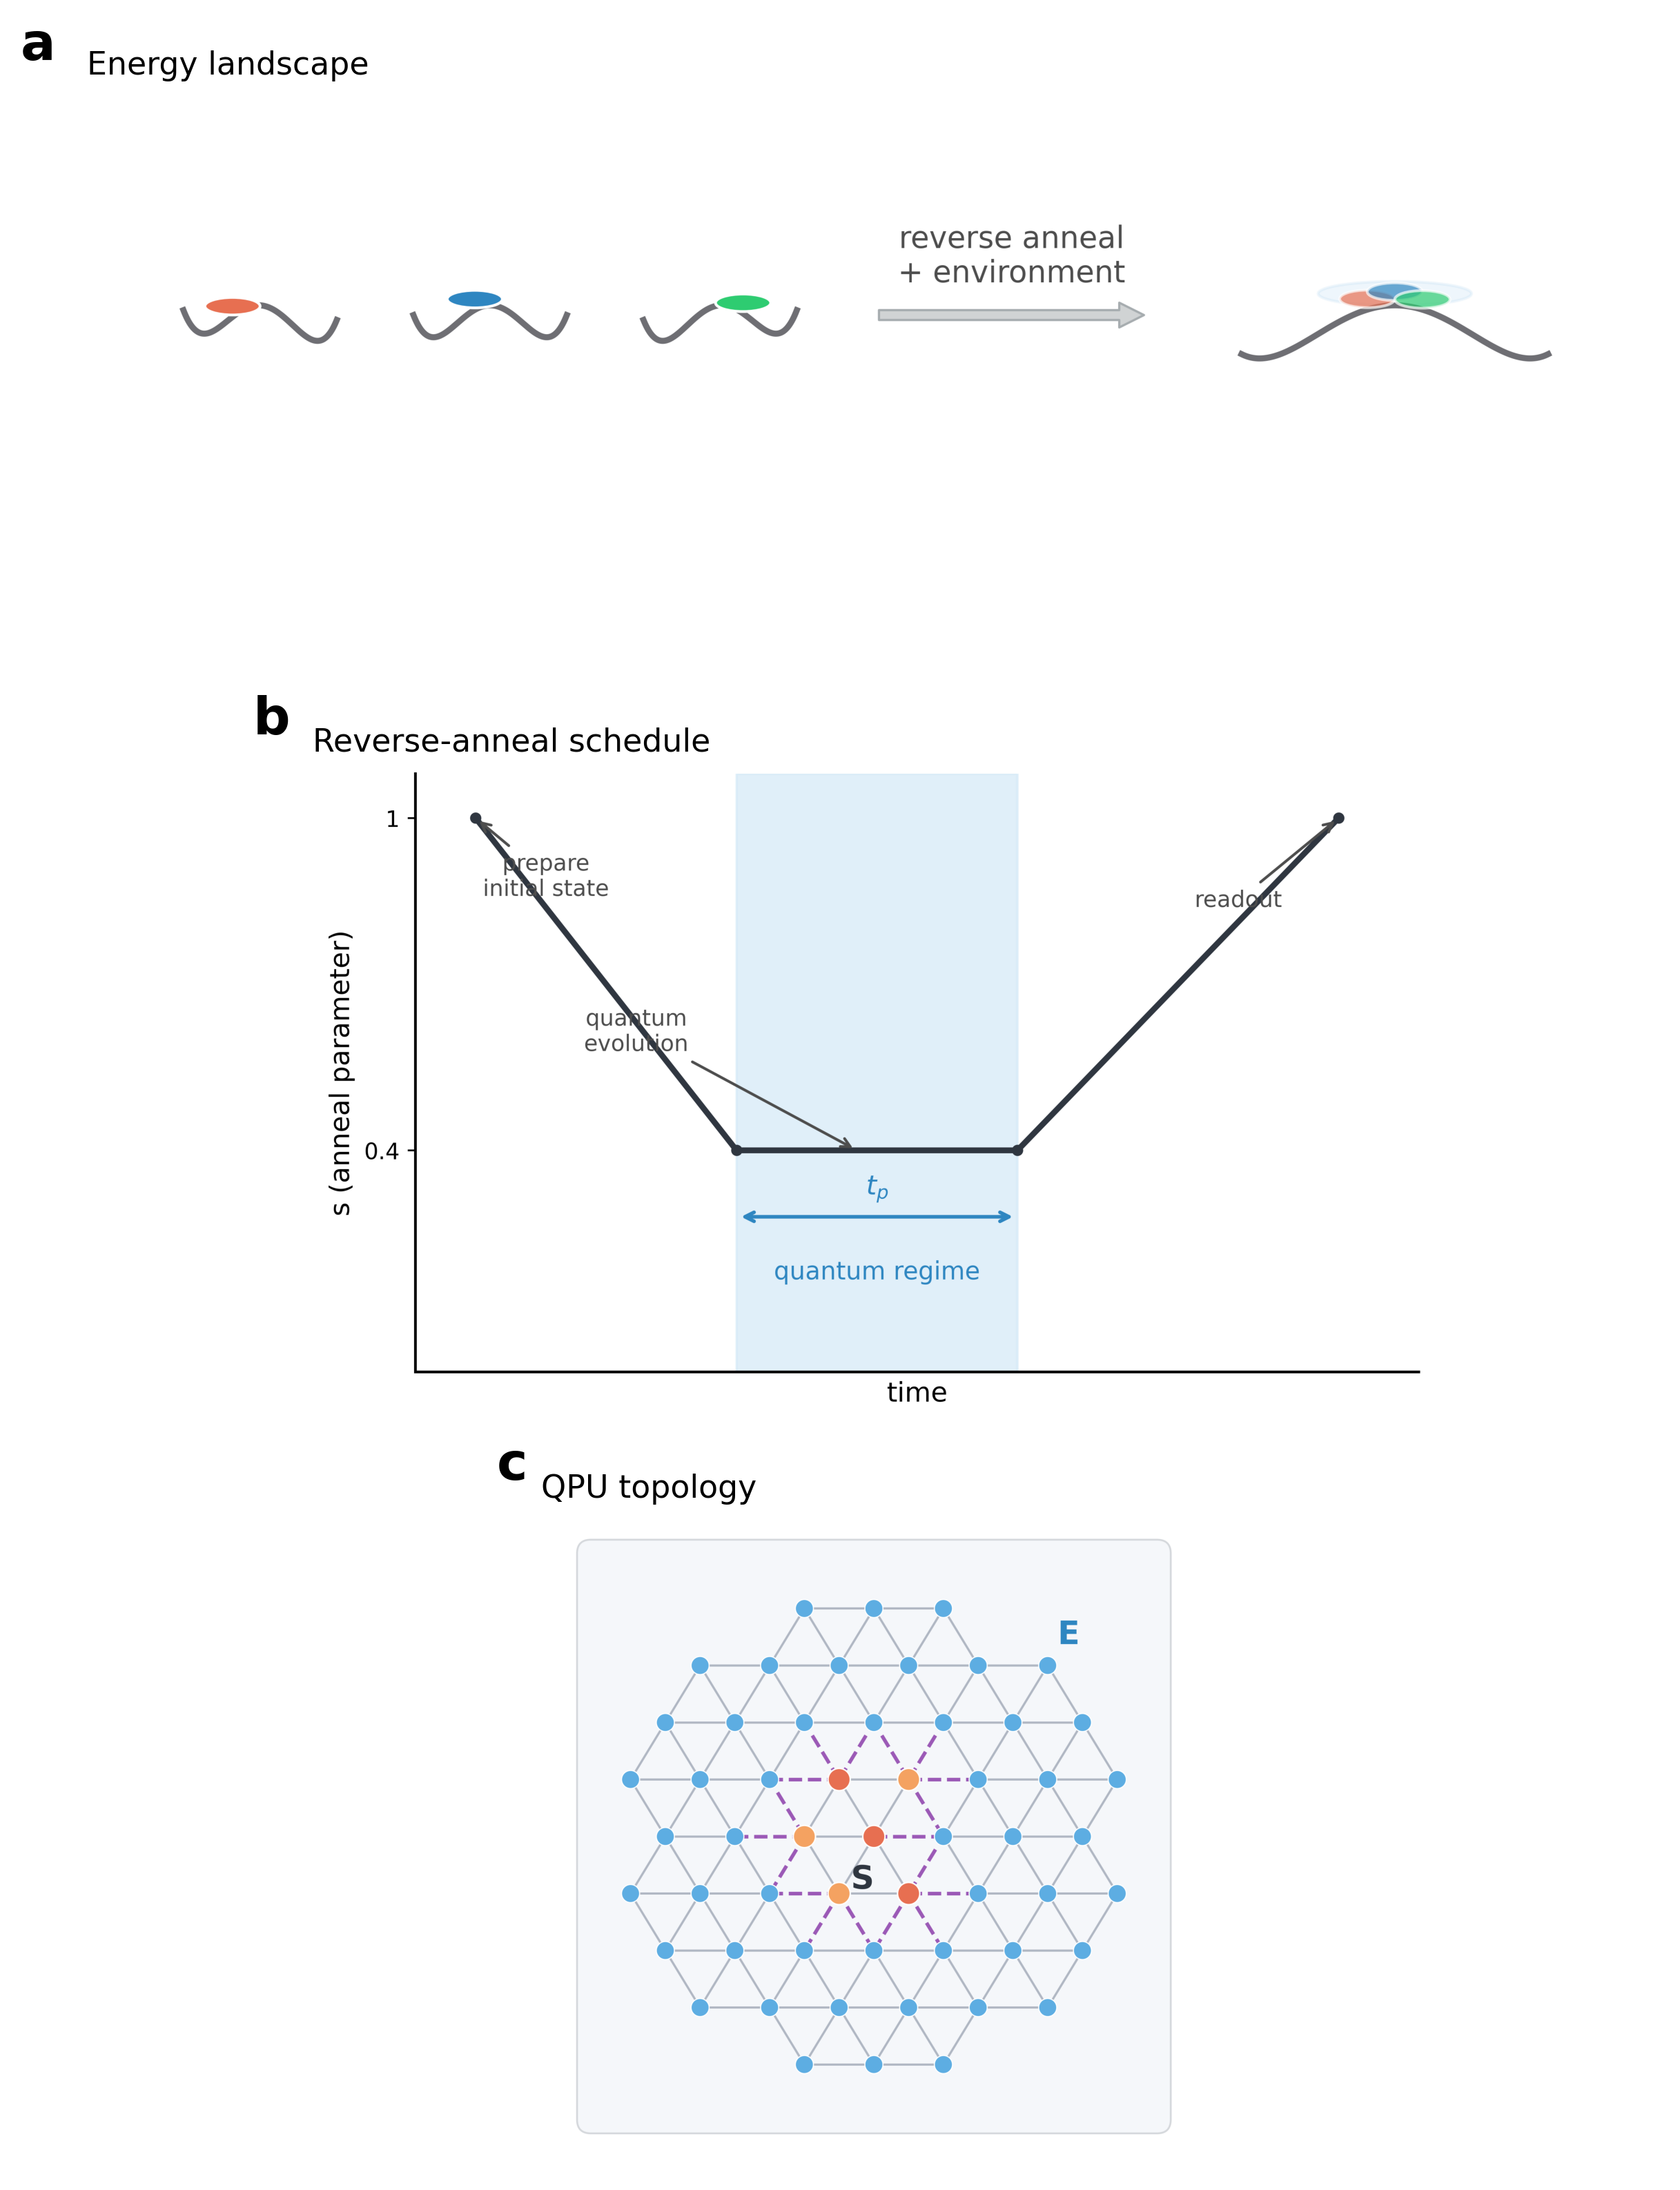
\includegraphics[width=\textwidth]{figures/fig1_combined.png}
\caption{\textbf{Reverse-anneal protocol and subsystem--environment partition.}
\textbf{a,}~Energy-landscape concept: three distinct initial preparations of the subsystem (colored balls in different potential wells) converge to the same distribution under relaxing conditions after reverse annealing in the presence of a large on-chip environment.
\textbf{b,}~Reverse-anneal schedule.  The system is initialized at $s=1$ (classical), ramped to a pause point $s_p$ where quantum fluctuations are reintroduced (blue-shaded region), held for a time $t_p$, and returned to $s=1$ for readout.
\textbf{c,}~Schematic of the subsystem--environment partition on the QPU topology.  The subsystem~$S$ (orange, $|S|=6$) is a connected cluster of qubits; the environment~$E$ (blue) surrounds it.  Dashed purple lines indicate the boundary couplers of programmable strength~$\lambda$.}
\label{fig:protocol}
\end{figure*}

Our experiment uses D-Wave's reverse-annealing protocol (Fig.~\ref{fig:protocol}b).
The QPU implements the time-dependent Hamiltonian $H(s) = -\frac{A(s)}{2}\sum_i \sigma_x^i + \frac{B(s)}{2}H_P$, where $H_P = \sum_i h_i \sigma_z^i + \sum_{ij} J_{ij}\sigma_z^i\sigma_z^j$ is the programmable problem Hamiltonian and $s\in[0,1]$ parameterizes the anneal~\cite{dwave2024reverse_anneal}.
In reverse annealing, the system is initialized in a classical state at $s=1$, ramped to a pause point~$s_p < 1$ where quantum fluctuations are reintroduced, held for a pause time~$t_p$, and returned to $s=1$ for readout.

We partition the qubits into a subsystem~$S$ ($|S|=6$) and an environment~$E$ ($|E|$ up to 50), connected through boundary couplers of strength~$\lambda$ (Fig.~\ref{fig:protocol}c).
Internal couplings are ferromagnetic ($J=-1$), and quenched disorder is introduced as random longitudinal fields $h_i\sim\mathcal{U}[-W,W]$.
Different initial preparations of~$S$ (all spins up, all down, or random) are used while holding~$E$ fixed.
The key observable is the memory order parameter~$\mathcal{M}$, defined as the maximum pairwise total variation distance (TVD) between the marginal distributions $P_S$ obtained from different initial states (see Methods).
$\mathcal{M}\to 0$ signals initial-state independence; $\mathcal{M}= 1$ indicates complete memory retention.

\subsection{Subsystem relaxation with tunable environment}

With the protocol and subsystem partition defined, we first show that enlarging and more strongly coupling the environment drives the subsystem toward initial-state independence within experimental resolution on both QPU generations (Fig.~\ref{fig:subsystem}).
On the Advantage2 QPU ($s_p=0.4$, $t_p=100\,\mu$s), the memory order parameter drops sharply with environment size: from $\mathcal{M}=1.0$ at $|E|=4$ to $\mathcal{M}=0.005$ at $|E|=8$ and $\mathcal{M}<0.005$ for $|E|\geq 16$ (Fig.~\ref{fig:subsystem}a, blue circles).
The Advantage\_system6.4 QPU shows the same qualitative trend, with a slightly higher residual memory at intermediate~$|E|$ consistent with its lower energy-to-temperature ratio (Fig.~\ref{fig:subsystem}a, red squares).

The coupling strength~$\lambda$ provides an independent control parameter (Fig.~\ref{fig:subsystem}b).
On Advantage2, memory decreases monotonically from $\mathcal{M}=0.94$ at $\lambda=0.05$ through $0.53$ at $\lambda=0.2$ to $\mathcal{M}<0.001$ for $\lambda\geq 0.3$.
On System~6.4, a similar crossover occurs at lower nominal~$\lambda$, illustrating that the threshold is platform- and submission-path-dependent rather than set by $\beta_\mathrm{eff}\lambda$ alone.
The submission-path dependence is itself quantifiable and reproducible: paired \texttt{auto\_scale} on/off repeats of the same $26$-qubit embedded problem in the transition region shift $\mathcal{M}$ from $\approx 0.99$ to $\approx 0.005$ ($\Delta\mathcal{M}\approx 0.98$, stable across four back-to-back repeats), while saturated conditions away from the crossover are unaffected (Methods; Supplemental Material)---so all absolute thresholds in this work are reported as empirical quantities for the stated submission path.

To probe the role of the pause-point Hamiltonian, we sweep~$s_p$ on both QPUs (Fig.~\ref{fig:subsystem}c,d).
The crossover curves display the same sigmoidal shape on both platforms: as $s_p$ increases from 0.35 to 0.50, the crossover coupling~$\lambda_c$ shifts to larger values, reflecting the decreasing transverse field.
In~situ single-qubit probes at $s_p=0.4$ yield $\beta_\mathrm{eff}=7.22\pm 0.06$ (Advantage2) and $\beta_\mathrm{eff}=4.29\pm 0.29$ (System~6.4) (Fig.~\ref{fig:disorder}c; see Methods), a ratio of $1.68$ consistent with the different hardware energy scales.
The common functional form across $s_p$ and the systematic threshold shift between QPUs suggest that pause-point Hamiltonian parameters are important, while platform-specific open-system contributions remain necessary to explain the full crossover; rescaling by $\beta_\mathrm{eff}^{\mathrm{S6.4}}/\beta_\mathrm{eff}^{\mathrm{A2}}\approx 0.59$ does not produce a single master curve, leaving a residual $\sim 3\times$ gap at $s_p=0.4$ that is not attributable to the transverse-field ratio $A(s_p)/B(s_p)$ (nearly identical at $0.260$ versus $0.259$) and is more naturally accommodated by platform-specific open-system contributions (flux-noise spectra, chain strength, calibration epoch, schedule outside the pause) that the dimensionless $\beta_\mathrm{eff}$ alone does not capture.
The cross-QPU comparison is anchored to a single $(s_p,t_p)=(0.4,\,100\,\mu\mathrm{s})$ operating point on each device, with $t_p$ set well above the relaxation timescale characterized in the kinetics scan; we did not separately sweep $t_p$ at $s_p=0.4$ on Advantage\_system6.4 (Supplemental Material).

\subsection{Environment-state dependence and kinetics}

We next ask which environment states produce this initial-state independence and on what timescale it develops.
At the relaxed working point ($|E|=50$, $\lambda=0.5$), an ordered $E$ (all-up or all-down) gives $\mathcal{M}=0.000$, while a random or domain-wall $E$ leaves residual memory $\mathcal{M}=0.39$ and $0.65$ respectively, with $P_S$ depending on which $E$ preparation was used (cross-preparation $\mathrm{TVD}=1.0$).
The on-chip environment is therefore a finite-size partner whose initial microstate influences the subsystem's fate, not a universal thermal bath.
Pause-time kinetics confirm that the ordered/disordered distinction is not a timescale effect: with ordered $E$, $\mathcal{M}$ drops from $0.017$ at $t_p=1\,\mu$s to $<0.001$ by $t_p=5\,\mu$s and remains zero to $t_p=500\,\mu$s, while with random $E$ it fluctuates between $0.1$ and $0.7$ over the same range with no systematic decay.
We adopt $t_p=100\,\mu$s ($\sim 20\times$ the ordered-$E$ relaxation timescale) as the working pause time for all subsequent campaigns.
A complementary test using $E$ states produced by forward-annealing the $E$-only Hamiltonian (with $S$ decoupled), which yields low-energy ordered samples, gives $\mathcal{M}=0.000$ across the tested preparations, consistent with the expectation~\cite{linden2009equilibration,popescu2006entanglement} that the environment's energy sector controls whether it acts as an effective bath.

\begin{figure*}[!htbp]
\centering
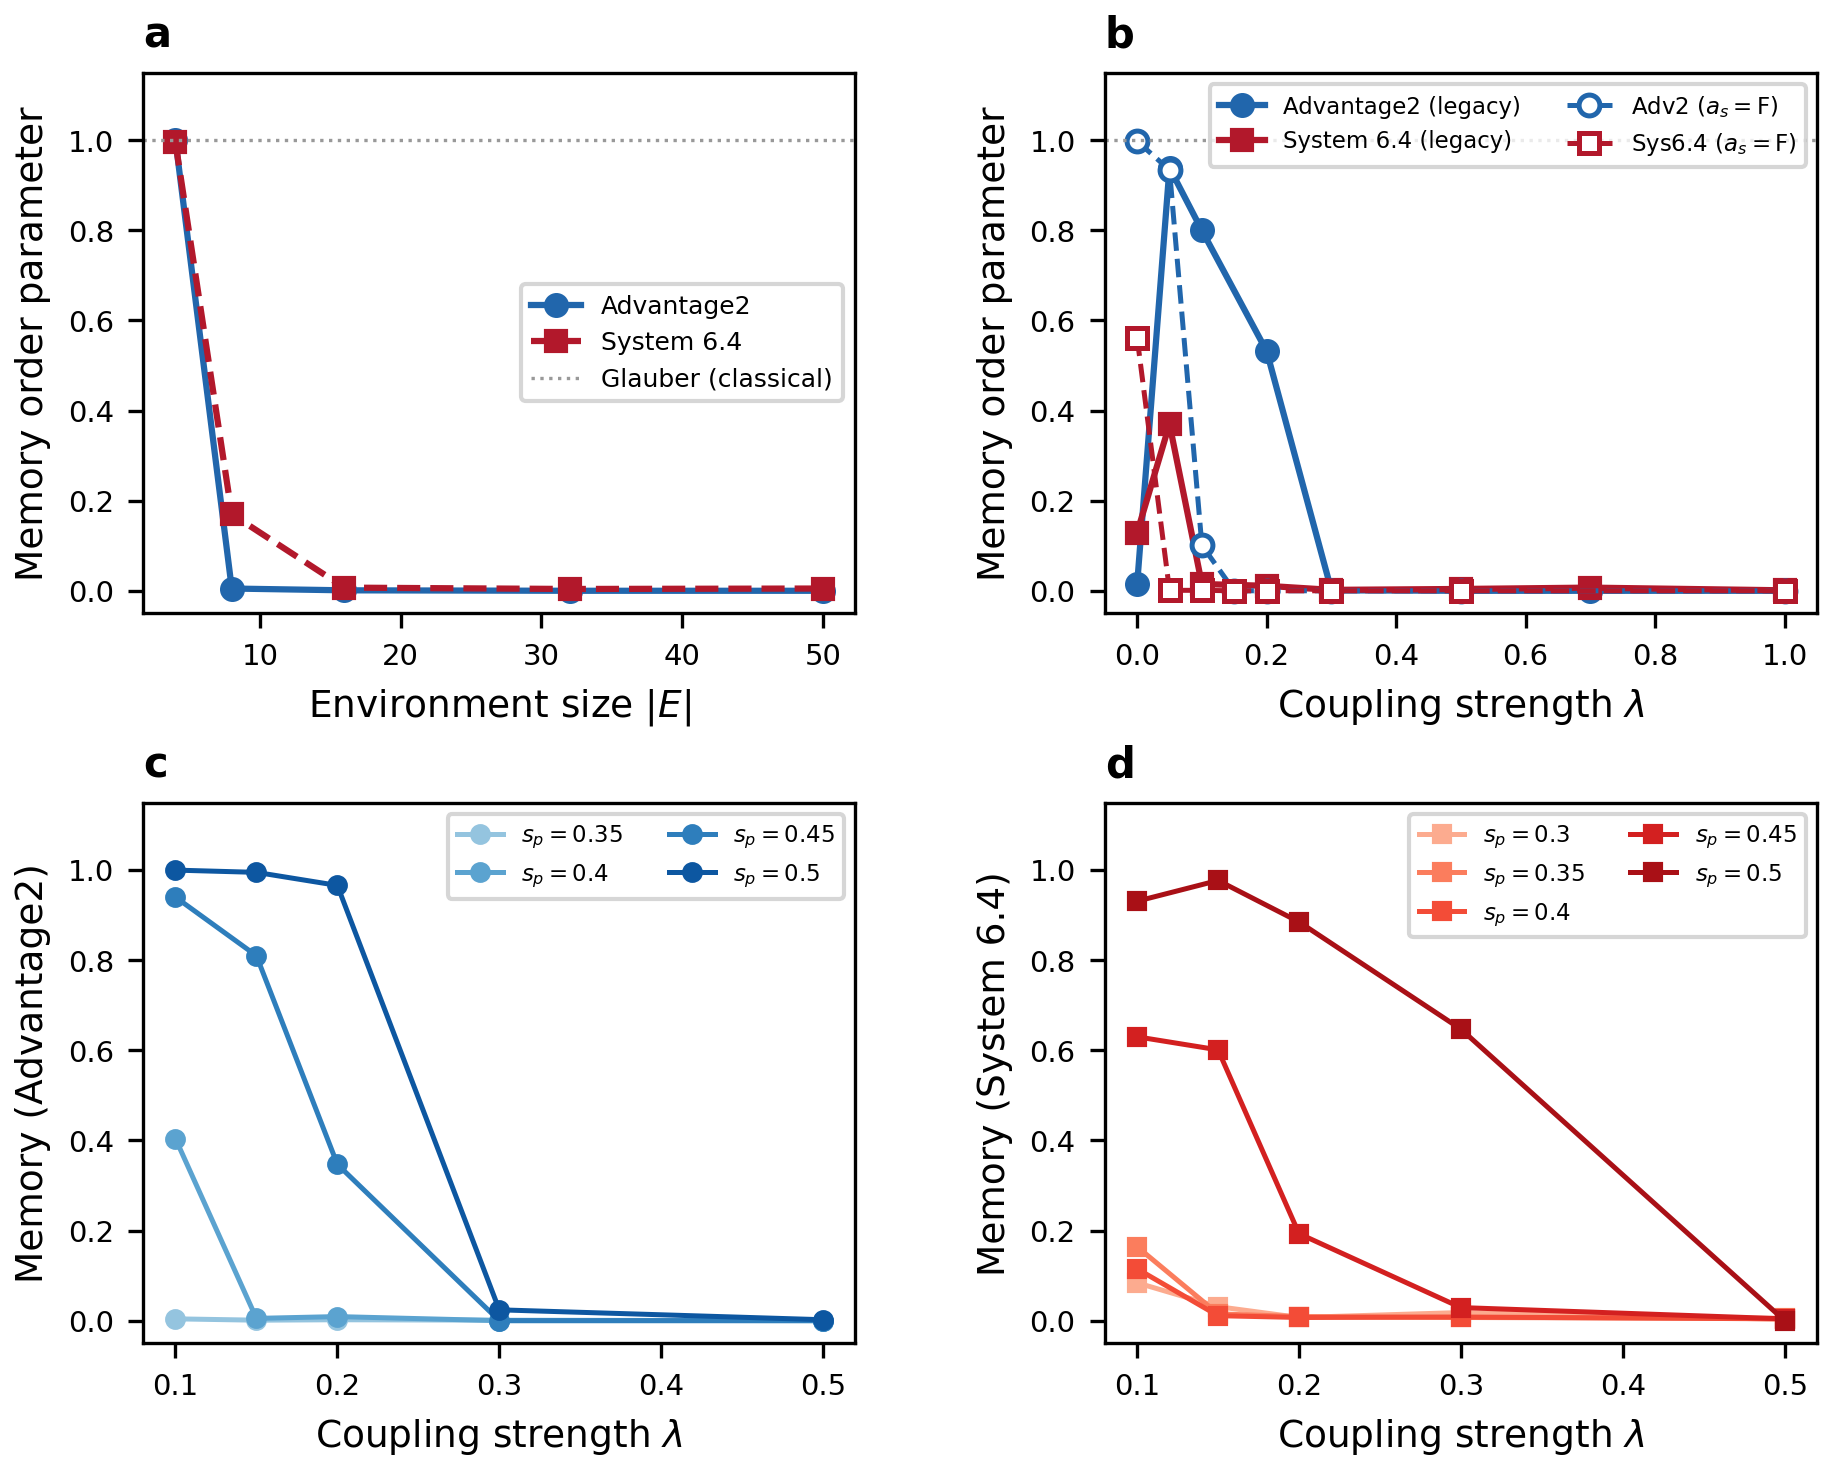
\includegraphics[width=\textwidth,height=0.55\textheight,keepaspectratio]{figures/fig3_subsystem.png}
\caption{\textbf{Bath size and coupling tune a memory-to-relaxation crossover, reproduced on both QPU generations.}
\textbf{a,}~Memory order parameter $\mathcal{M}$ versus environment size $|E|$ on both QPUs ($s_p=0.4$, $\lambda=0.5$).
\textbf{b,}~Memory versus coupling strength $\lambda$ ($|E|=50$).  Filled markers with solid lines: legacy SDK-default submission path.  Open markers with dashed lines: regenerated on direct native-qubit submissions with \texttt{auto\_scale=False} (no chain couplers).  The $\lambda=0$ point is a decoupled control and is excluded from the monotonic crossover statement.
\textbf{c,d,}~Pause-depth sweeps on Advantage2 (\textbf{c}) and System~6.4 (\textbf{d}); lower $s_p$ shifts relaxation to weaker coupling.
Plotted threshold values are nominal SDK-default quantities and inherit the \texttt{auto\_scale} systematic characterized in Methods and the Supplemental Material; bootstrap error bars are smaller than the markers unless shown.}
\label{fig:subsystem}
\end{figure*}

\subsection{Disorder as a control parameter for relaxation}

The sensitivity to the environment's initial energy sector suggests that disorder should compete directly with the same relaxation mechanism, making quenched disorder a third control knob---alongside bath size and coupling---that a sampler user must account for; we test it by adding random longitudinal fields (Fig.~\ref{fig:disorder}a).
At fixed $|E|=50$ and $\lambda=0.5$, $\mathcal{M}$ remains near zero for $W\leq 1.0$ on both QPUs and then rises above the noise floor for a subset of disorder realizations beyond $W\approx 1.5$, reaching single-realization values of $\mathcal{M}=0.74$ at $W=2.0$ on Advantage2 and $\mathcal{M}=0.50$ at $W=1.5$ on System~6.4, the lower threshold consistent with its smaller $\beta_\mathrm{eff}$.
The effect is realization-dependent: a five-realization disorder average on Advantage2 gives $\mathcal{M}=0.000\pm 0.000$ for $W\leq 1.0$, $0.001\pm 0.001$ at $W=1.5$, and $0.125\pm 0.103$ at $W=2.0$, where the dispersion as large as the mean (5 seeds) indicates that some realizations arrest while most do not.
The full $(\lambda, W)$ crossover diagram on Advantage2 (Fig.~\ref{fig:disorder}b, 72 grid points) reveals, at the single system size studied ($|S|=6$, $|E|=50$), an empirical boundary separating initial-state-independent and memory-retaining regions, with stronger coupling pushing the disorder threshold higher; absent a finite-size scaling analysis we treat this as a single-size threshold, not a thermodynamic phase boundary.
The disorder-arrest threshold is graph-dependent: native Zephyr subgraphs, whose boundary connectivity is roughly an order of magnitude denser than the random 3-regular logical graphs studied here, relax across a broader range of $W$ (Supplemental Material).
The lower-connectivity logical graph therefore provides a more stringent test of disorder arrest. We note only in passing that the open-system nature of the QPU and the finite pause time preclude any identification with a many-body-localization transition, despite a superficial resemblance; the operational point is simply that disorder above $W\approx 1.5$ degrades relaxation and must be logged as a sampler-validation parameter.

\begin{figure*}[!htbp]
\centering
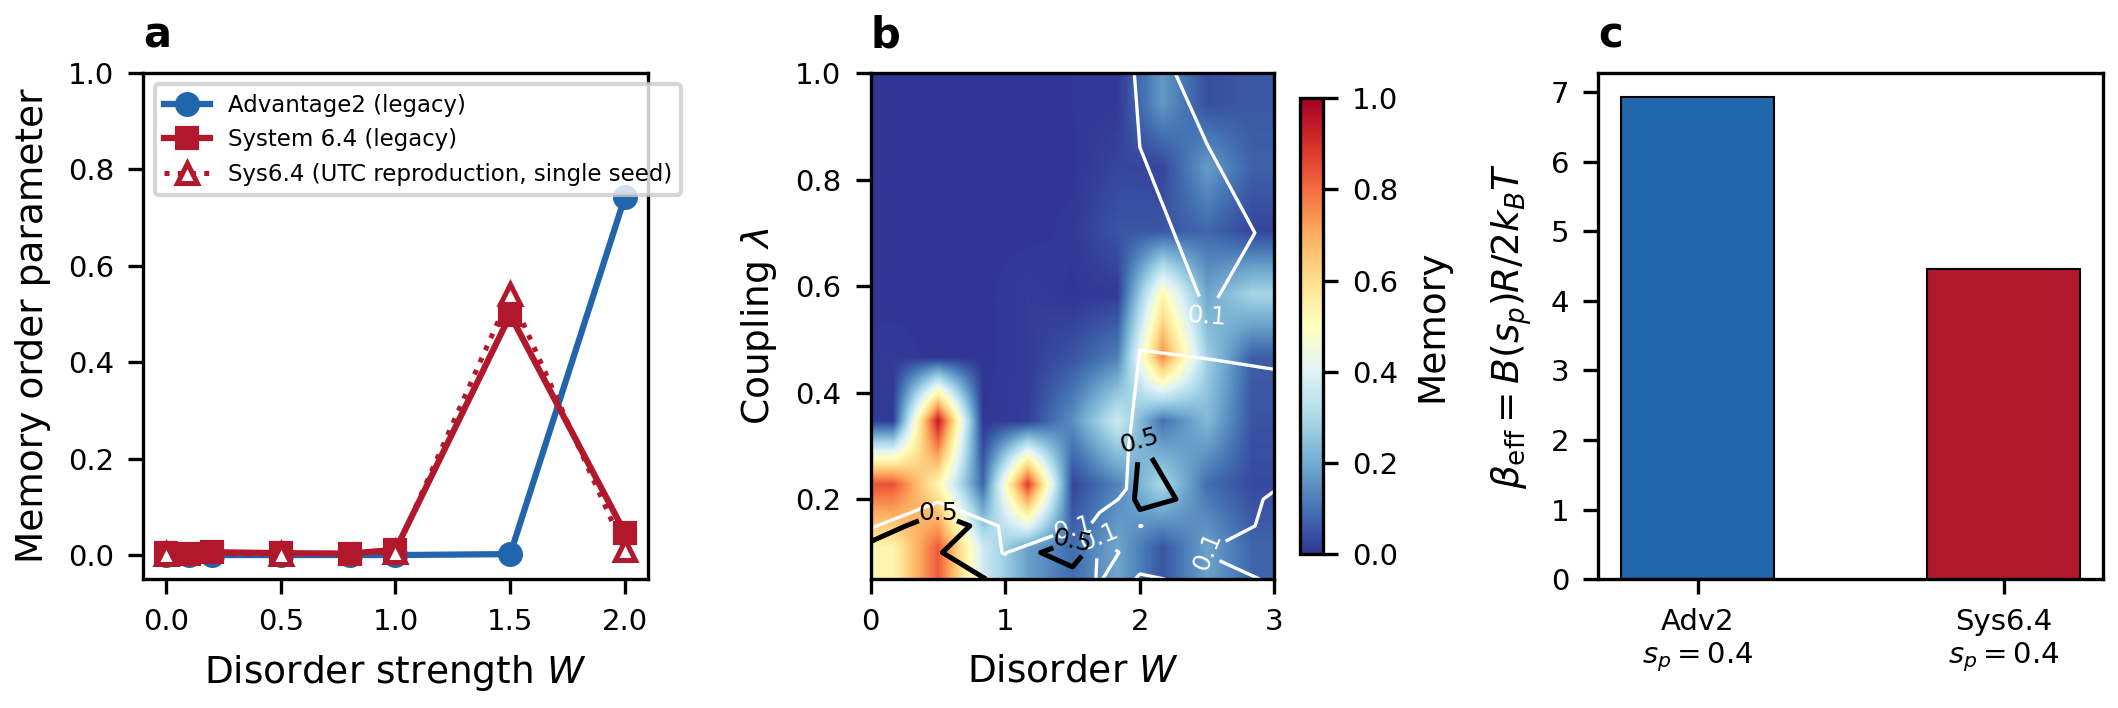
\includegraphics[width=\textwidth,height=0.55\textheight,keepaspectratio]{figures/fig4_disorder.png}
\caption{\textbf{Disorder degrades relaxation above $W\approx 1.5$.}
\textbf{a,}~Memory order parameter versus disorder strength~$W$ on both QPUs ($|E|=50$, $\lambda=0.5$, $s_p=0.4$).  Solid curves: legacy SDK-default submission path.  Open triangles (dotted, red): a single-seed reproduction on \texttt{Advantage\_system6.4} at the \texttt{uniform\_torque\_compensation} chain-strength path with \texttt{auto\_scale=True}, giving $\mathcal{M}=0.54$ at $W=1.5$ versus the legacy $0.50$.  Memory rises above the noise floor for a subset of realizations beyond $W\approx 1.5$--$2.0$ (5-seed average $\mathcal{M}=0.125\pm 0.103$ at $W=2.0$); the lower threshold on System~6.4 is consistent with its smaller~$\beta_\mathrm{eff}$.  Smaller fixed chain strengths (Supplemental Material) give weaker arrest, so the arrest magnitude here is specific to the legacy chain-strength regime.
\textbf{b,}~Single-size empirical crossover in the $(\text{disorder}\;W,\;\text{coupling}\;\lambda)$ plane on Advantage2 (72 grid points, $|E|=50$, $|S|=6$).  Color indicates $\mathcal{M}$; contour lines at $\mathcal{M}=0.1$ (white) and $0.5$ (black) delineate the relaxed and memory-retaining regions at this single system size (not a thermodynamic phase diagram).  Stronger coupling pushes the disorder threshold higher.
\textbf{c,}~In~situ measured dimensionless energy scale $\beta_\mathrm{eff}=B(s_p)R/2k_BT$ at $s_p=0.4$ on both QPUs.}
\label{fig:disorder}
\end{figure*}

\subsection*{Effective thermal marginal}

Having established when the subsystem relaxes, we next ask what distribution the relaxed subsystem approaches.
The subsystem-relaxation measurements above show that, in the relaxed
regime defined by the memory order parameter, the measured subsystem
distribution becomes nearly independent of the initial subsystem state.
They do not by themselves determine whether the common distribution has a
thermal form.  We therefore compare the measured marginal $P_S$ with a
classical conditional Boltzmann marginal evaluated at an effective inverse
temperature calibrated on independent one-qubit probes.

\paragraph{In-situ $\beta_\mathrm{eff}$ calibration.}
Following the spirit of classical thermometry protocols for quantum
annealers~\cite{grattan2025thermometry}, we define $\beta_\mathrm{eff}$
operationally as the Boltzmann slope of the $z$-basis readout distribution
produced by the complete reverse-anneal protocol on a single-qubit probe.  We submit Ising problems consisting of
one active qubit with longitudinal bias $h=0.5$ and no couplings, use the
same reverse-anneal schedule as the many-body experiment
($s_p=0.4$, $t_p=100\,\mu$s, \texttt{auto\_scale=False}, 5{,}000 reads per
initial state), and estimate
\begin{equation}
    \beta_\mathrm{eff}
    = \frac{1}{2h}
      \ln\!\left(\frac{n_\downarrow}{n_\uparrow}\right),
    \label{eq:beta_eff}
\end{equation}
with the result averaged over three probe qubits drawn from the solver
nodelist.  For the main thermal-marginal sweep on Advantage2
(native exact-enumeration, random-regular exact-enumeration, Hamiltonian-scale, large-bath and disorder sub-experiments), taken after
the Advantage2 solver rename and recalibration, this procedure gives
$\beta_\mathrm{eff}=7.219\pm0.063$ at $s_p=0.4$; the frustrated pilot
described below was submitted in a separate run and uses an independently
recalibrated $\beta_\mathrm{eff}=7.331\pm0.198$.  For the
Advantage\_system6.4 cross-QPU replication the same procedure gives
$\beta_\mathrm{eff}=4.289\pm0.294$.  All three values should be
distinguished from the earlier main-experiment calibration of
$\beta_\mathrm{eff}=6.93\pm0.20$ (Advantage2) and
$4.46\pm0.26$ (Advantage\_system6.4) quoted elsewhere in the paper.  In
every case, $\beta_\mathrm{eff}$ is a protocol-level readout parameter:
it is not identified with the refrigerator temperature, nor with a
quantum Gibbs temperature of the pause-point Hamiltonian.

\paragraph{Conditional Gibbs prediction.}
For the thermal-marginal data analyzed here, the environment is prepared in
a fixed ordered state.  The corresponding classical target for the
subsystem is therefore the conditional marginal
\begin{equation}
    P_S^\mathrm{th}(\sigma_S \mid \sigma_E = \mathbf{1})
    =
    \frac{
        \exp[-\beta_\mathrm{eff}
        H_P(\sigma_S,\sigma_E=\mathbf{1})]
    }{
        \sum_{\sigma_S'}
        \exp[-\beta_\mathrm{eff}
        H_P(\sigma_S',\sigma_E=\mathbf{1})]
    },
    \label{eq:cond_gibbs}
\end{equation}
which we evaluate by direct enumeration of the $2^{|S|}$ subsystem
configurations with $\sigma_E$ held fixed.  This conditional object differs
from an unconditional equilibrium marginal, which averages over environment
configurations and therefore does not encode the prepared symmetry-breaking
boundary condition.  In globally spin-flip-symmetric instances, the
unconditional marginal would average over the two ordered sectors and
predict zero subsystem magnetization.

\paragraph{Main result.}
In a 10-seed disorder sweep at fixed $N=12$, $|S|=4$, $\lambda=0.5$ on a
3-regular logical graph (Fig.~\ref{fig:thermal_marginal}), the measured marginal agrees with the
conditional classical prediction whenever the memory criterion identifies
the instance as relaxed.  Over the tested values
$W\in\{0,0.25,0.5,0.75,1.0,1.25\}$, the mean
$D_\mathrm{TV}(P_S^\mathrm{exp},P_S^\mathrm{th})$ over relaxed disorder
realisations lies between
$0.6\times10^{-3}$ and $3.6\times10^{-3}$, below the estimated
multinomial sampling floor for this comparison and with no clear monotone
dependence on $W$ (Fig.~\ref{fig:thermal_marginal}b).  In the same sweep, the fraction of relaxed
disorder realisations decreases from $10/10$ at $W=0$ to $4/10$ at $W=1.25$
(Fig.~\ref{fig:thermal_marginal}a), consistent with the disorder-induced arrest reported above.
Thus, within this sweep, disorder primarily controls whether the subsystem
reaches the common marginal; conditioned on relaxation, the common marginal
is consistent with the calibrated conditional Boltzmann form.

The same diagnostic gives the same qualitative conclusion at the
main-experimental scale.  For $|S|=6$, $|E|=50$ on native Zephyr
subgraphs, $11/14$ conditions are relaxed across the two Hamiltonian
scales ($5/7$ unscaled and $6/7$ at scale $0.5$), and every one of
those $11$ relaxed conditions satisfies
$D_\mathrm{TV}<10^{-3}$ against the classical conditional target, with
maxima $5.0\times10^{-4}$ and $2.6\times10^{-4}$ in the two sets
respectively.  Across the full $494$-condition thermal-marginal sweep on
Advantage2 (native Zephyr, random 3-regular, three Hamiltonian scales,
large-bath native and disorder sub-experiments), $113/494$ conditions satisfy the relaxation
criterion, and all but three of them have classical conditional
$D_\mathrm{TV}$ below $0.05$; the three exceptions are the two severe
wrong-basin trapping instances and one borderline miss described below.
An independent $60$-condition cross-QPU replication on
Advantage\_system6.4 agrees qualitatively: $22/60$ instances satisfy
$\mathcal{M}\le0.05$ at the separately calibrated
$\beta_\mathrm{eff}=4.29$, with classical conditional $D_\mathrm{TV}$
distributed over $[3\times10^{-5},\,0.029]$ and median $0.005$.  These
passing conditions span graph geometry (random 3-regular and native
Zephyr), subsystem size ($|S|\in\{4,6\}$), coupling strength
($\lambda\in\{0.2,0.3,0.5\}$), and Hamiltonian energy scale (overall
factors $0.35$, $0.5$, $0.75$, and $1.0$).  The comparison therefore
provides a thermal-marginal test that is separate from, and stricter
than, loss of initial-state memory alone (Fig.~\ref{fig:thermal_marginal}c).

\paragraph{Quantum reduced Gibbs diagnostic.}
The same comparison can be repeated with the $z$-basis diagonal of the
quantum reduced Gibbs state of the pause-point Hamiltonian,
\begin{equation}
    H(s_p)
    =
    -\frac{A(s_p)}{2}\sum_i \sigma_x^i
    + \frac{B(s_p)}{2} H_P ,
    \label{eq:Hsp}
\end{equation}
evaluated on the full $N$-qubit system by exact diagonalisation for
$N\le12$, with the transverse field retained at $s_p$.  We use the same
protocol-level $\beta_\mathrm{eff}$ and the device-calibrated ratio
$A(s_p)/B(s_p)=0.260$ for Advantage2 and $0.259$ for
Advantage\_system6.4, extracted directly from the solver anneal-schedule
spreadsheets at $s_p=0.4$.  Two quantum targets are compared against the
pooled measured marginal: the \emph{conditional} quantum reduced Gibbs
marginal with $\sigma_E$ fixed to the prepared ordered state, and the
\emph{unconditional} marginal that traces over all $2^{|E|}$ environment
configurations.

The conditional quantum reduced Gibbs target is tight in the disorder
sweep but not uniformly across all scaled ferromagnetic
conditions.  On this disorder sweep at $N=12$, $|S|=4$, $\lambda=0.5$ on
a 3-regular logical graph, the median conditional quantum
$D_\mathrm{TV}$ across 43 relaxed Advantage2 conditions is $0.0145$
(max $0.0272$); on the 22 relaxed Advantage\_system6.4 conditions it is
$0.0146$ (max $0.0284$).  Across the 102 relaxed $N\le12$ ferromagnetic
main-sweep conditions for which the quantum target was computed,
$73$ satisfy $D_\mathrm{TV}\le0.05$ and $29$ exceed it, with the excesses
concentrated in the Hamiltonian-scale sweeps.  Scaling the problem
Hamiltonian by a factor $s$ leaves $A(s_p)$ unchanged but multiplies
$B(s_p)H_P$ by $s$, so the effective transverse-to-longitudinal ratio
seen by the reduced Gibbs state is $A/(sB)$; at scale $0.35$
this is $0.260/0.35\approx0.74$, at scale $0.5$ it is
$0.260/0.5\approx0.52$, and at scale $0.75$ it is
$0.260/0.75\approx0.35$.  The conditional quantum diagonal therefore
accumulates increasingly large transverse-field-induced excited-state
mixing at smaller scale, mixing that the measured post-return-ramp
readout does not display.  The unconditional quantum reduced Gibbs
marginal is a much worse target in every ferromagnetic regime (median
$D_\mathrm{TV}\approx 0.5$ in the Advantage2 disorder sweep), which is
expected because the unconditional marginal averages over both ordered
sectors of the global $Z_2$ and cannot encode the prepared all-up
boundary.

The residual gap between the classical and conditional quantum
predictions in the ferromagnetic regime is consistent with the
interpretation of the calibrated $\beta_\mathrm{eff}$ as a
protocol-level readout slope: the readout distribution is measured
after the return ramp to $s=1$, and the net protocol-level mapping
from the reverse anneal, pause, return ramp and readout absorbs the
small transverse-field-induced mixing that the conditional quantum
pause-point state would otherwise carry.  Within that single
$\beta_\mathrm{eff}$, both the classical and quantum conditional
predictions are consistent with the measurements, with the classical
conditional target the tighter of the two.

A frustrated pilot, in which the sign of each coupler is flipped with
probability $\tfrac12$ (Edwards--Anderson bond disorder) on top of the
random 3-regular $N=12$, $|S|=4$, $\lambda=0.5$ sweep at five disorder
seeds, inverts that ordering.  On the two conditions that satisfy
$\mathcal{M}\le0.05$, the classical conditional target has
$D_\mathrm{TV}=0.32$ on average (max $0.64$), while the conditional
quantum reduced Gibbs target has $D_\mathrm{TV}=0.029$ on average (max
$0.045$): an order-of-magnitude-tighter agreement in this small relaxed subset.
This pilot suggests that the frustrated regime can distinguish the two
predictions in the multi-modal classical-marginal regime, but a larger
frustrated campaign is needed to establish the effect.  The evidence
for quantum effects in the main paper continues to enter primarily
through the relaxation dynamics---including the $s_p$-dependent
relaxation trends and the failure of device-temperature Glauber
dynamics to reproduce the observed initial-state mixing.  In the
ferromagnetic regime, the final relaxed $z$-basis weights are
consistent with either reduced Gibbs target at the same
$\beta_\mathrm{eff}$; the frustrated pilot instead favours the
conditional quantum target by roughly an order of magnitude on its
two relaxed instances, but this subset is too small to establish the
effect and motivates a dedicated frustrated campaign.

\paragraph{Dynamical-trapping failure modes.}
Three relaxed conditions in the 494-instance thermal-marginal sweep fail
the thermal-marginal test against the classical conditional target at
$D_\mathrm{TV}>0.05$.  Two of them are severe wrong-basin failures
corresponding to the same physical instance, $\lambda=0.2$, $N=8$,
$W=1.0$, seed~42 on a native Zephyr subgraph, observed at two
Hamiltonian scales.  At scale $0.35$ the memory order parameter is
$\mathcal{M}=0.0145$, the classical conditional
$D_\mathrm{TV}(P_S^\mathrm{exp},P_S^\mathrm{th})=0.9409$, and the
conditional quantum reduced Gibbs $D_\mathrm{TV}=0.5414$; at scale $0.5$
the corresponding values are $\mathcal{M}=0.0240$,
$D_\mathrm{TV}(\mathrm{classical})=0.9674$, and
$D_\mathrm{TV}(\mathrm{quantum~cond.})=0.3565$.  A third relaxed
condition with the same $(\lambda,N,W)$ but seed~123 at scale $0.35$ is
a borderline miss rather than a wrong-basin trap
($\mathcal{M}=0.0085$, $D_\mathrm{TV}=0.0513$), with measured
magnetisation close to $+1$ on every subsystem site.

For the severe scale-$0.5$ trapping instance, the three initial
subsystem states converge to nearly the same measured distribution, but
that distribution places $98.5\%$ of its weight on the higher-energy
all-down basin rather than on the classical all-up ground state.  Direct
enumeration of the conditional classical energies in the scaled units
gives $E_\uparrow=-1.7142$ and $E_\downarrow=-1.1675$, so at
$\beta_\mathrm{eff}=7.219$ the classical Boltzmann weight favours the
all-up basin by
$\exp[\beta_\mathrm{eff}(E_\downarrow-E_\uparrow)]\approx 52$.  The
scale-$0.35$ twin shows the same all-down localisation with
$\mathcal{M}=0.0145$.

Both wrong-basin instances are therefore consistent with dynamical
trapping into a common non-thermal basin rather than with incomplete
relaxation: the memory order parameter is below the relaxation
threshold in each case, but the converged distribution does not match
either the classical conditional or the conditional quantum reduced
Gibbs target.  Reporting the memory order parameter and the
thermal-marginal distance as two independent quantities separates
ordinary relaxation from this failure mode, and identifies the same
trapping pair whether the thermal target is the classical conditional
or the conditional quantum reduced Gibbs marginal.

The same comparison also acts as a diagnostic outside the relaxed regime,
though low pooled $D_\mathrm{TV}$ is not equivalent to relaxation.
Among the $381$ memory-retaining thermal-marginal conditions with $\mathcal{M}>0.05$,
the classical conditional distance against the prepared-$E$ target
spans $[0.003, 0.97]$ with median $0.35$; larger memory is generally
accompanied by larger deviation from the conditional Gibbs prediction,
but $22/381$ memory-retaining conditions have $D_\mathrm{TV}<0.05$
because the three-initial-state pooled marginal can accidentally
resemble the conditional target even when the individual initial-state
distributions remain distinct.  Reporting $\mathcal{M}$ and
$D_\mathrm{TV}$ together therefore separates ordinary relaxation to the
thermal marginal, the small number of relaxed-but-non-thermal trapping
instances, and these memory-retaining accidental-pool matches, and the
classification is stable under the corrected device-calibrated
$A(s_p)/B(s_p)$.

\begin{figure*}[!htbp]
\centering
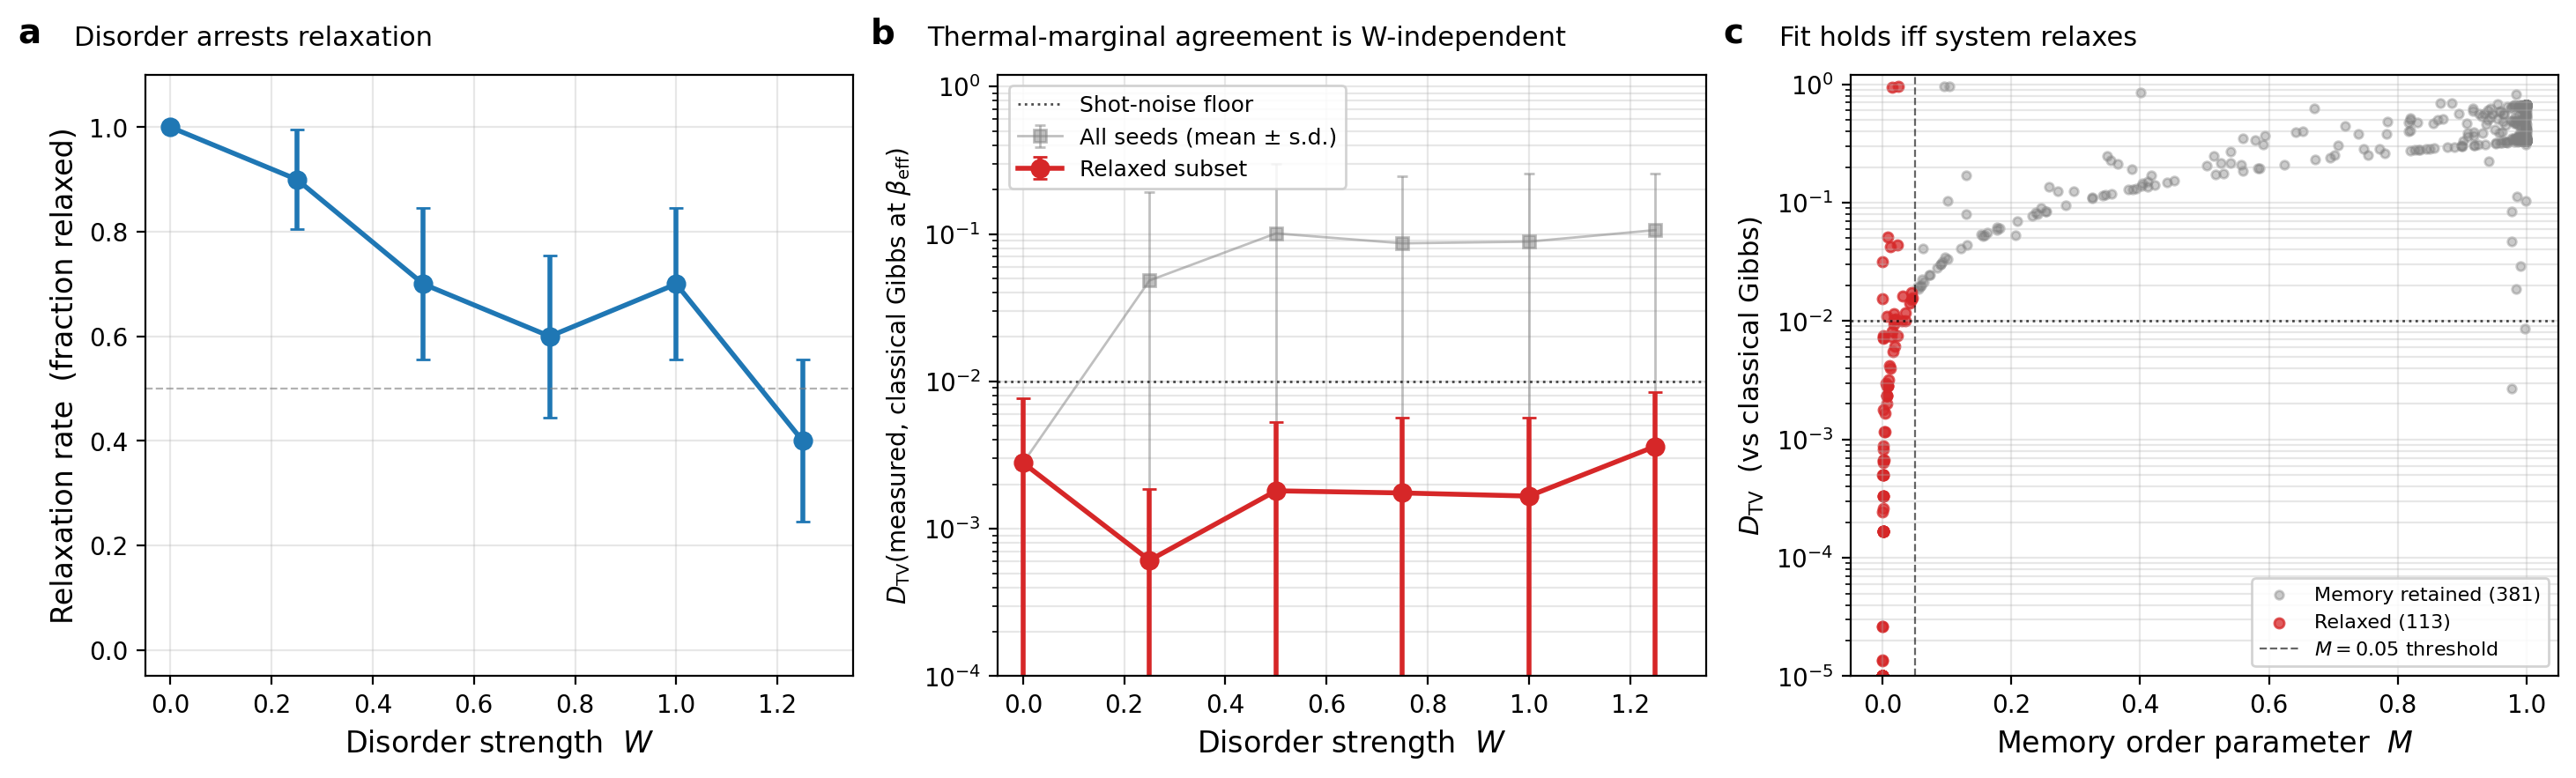
\includegraphics[width=\textwidth,height=0.72\textheight,keepaspectratio]{figures/fig6_thermal_marginal.pdf}
\caption{\textbf{Effective thermal marginal.}
\textbf{a,}~Fraction of relaxed disorder realisations ($\mathcal{M}\le 0.05$) in the 10-seed disorder sweep ($N=12$, $|S|=4$, $\lambda=0.5$, 3-regular logical graph, Advantage2).  Relaxation fraction decreases from $10/10$ at $W=0$ to $4/10$ at $W=1.25$.
\textbf{b,}~Total-variation distance between the pooled subsystem marginal and the calibrated classical conditional Gibbs target at $\beta_\mathrm{eff}=7.219$ vs disorder strength.  Open circles: all 10 seeds; filled circles: relaxed subset only (error bars = s.d. across relaxed seeds).  Grey band: finite-shot reference $D_\mathrm{TV}\simeq\tfrac12\sqrt{K/N_\mathrm{reads}}\approx 0.026$ with $N_\mathrm{reads}=6000$, $K=2^{|S|}=16$; the relaxed subset stays at or below this scale across the sweep.
\textbf{c,}~Scatter of $D_\mathrm{TV}$ vs $\mathcal{M}$ across all thermal-marginal conditions.  Red: relaxed ($\mathcal{M}\le 0.05$); grey: memory-retaining.  Two top-left red outliers correspond to the same $\lambda=0.2$, $N=8$, $W=1$, seed~42 native Zephyr instance at Hamiltonian scales $0.35$ and $0.5$ (dynamical trapping, discussed in the body).  The memory and thermal-marginal criteria identify the same condition set apart from this trapping pair and one borderline $D_\mathrm{TV}=0.051$ miss.}
\label{fig:thermal_marginal}
\end{figure*}


\subsection{Classical and small-system controls}

We next compare the relaxation crossovers and thermal-marginal endpoint against classical and small-system quantum controls (Fig.~\ref{fig:baselines}).
Single-spin-flip Glauber dynamics at the calibrated readout temperature $T_\mathrm{cal}=1/\beta_\mathrm{eff}$ (in the dimensionless coupling units; see Methods), and continuous-spin $O(3)$ spin-vector Monte Carlo~\cite{shin2014svmc}, both give $\mathcal{M}=1.0$ across the experimental ranges of system size, coupling strength, and disorder (Fig.~\ref{fig:baselines}a; Supplemental Material).
Exact diagonalization (ED) of the closed quantum Hamiltonian for $N\in\{8,10,12\}$ ($|S|=4$) is consistent with transverse-field-driven relaxation on the three ED-accessible sizes: at $s_p=0.4$, $t_p=0.5\,\mu$s, $\mathcal{M}$ falls from $0.47$ at $N=8$ to $0.13$ at $N=12$ (Fig.~\ref{fig:baselines}b); at $s_p=0.5$, $\mathcal{M}$ remains above $0.94$ at all sizes.
A complementary Lindblad master equation with local thermal jump operators at the calibrated readout temperature reproduces the same qualitative trend (Supplemental Material).
That both a closed-system (ED) and an open-system (Lindblad) model reproduce the trend indicates the qualitative crossover does not by itself discriminate coherent from dissipative dynamics; the agreement does not establish that the QPU dynamics are unitary, and is only consistent with the pause-point transverse field influencing small-system relaxation~\cite{mehta2025dwave}.
On both QPUs, the threshold coupling $\lambda_c$ shifts systematically with $s_p$ (Fig.~\ref{fig:baselines}c), with deeper pauses producing relaxation at weaker coupling---an $s_p$ dependence absent from any purely classical-$H_P$ dynamics, but one we do not over-read: $s_p$ simultaneously sets the transverse field $A(s_p)$, the problem prefactor $B(s_p)$ and the $s_p$-dependent open-system rates, which we do not separately isolate.

\begin{figure*}[!htbp]
\centering
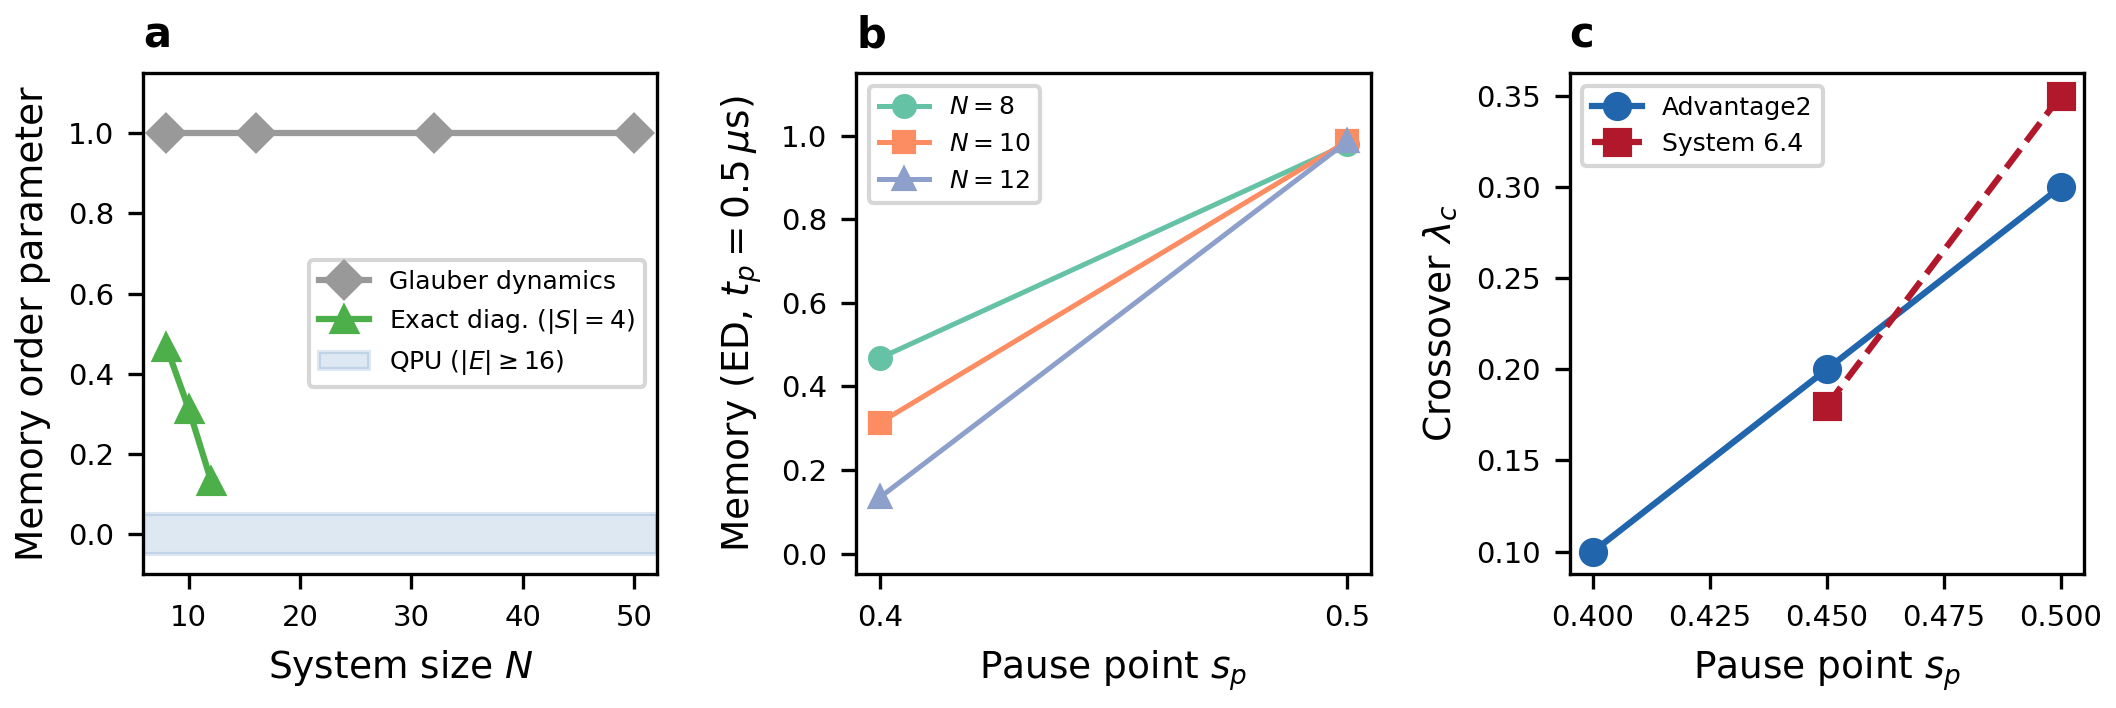
\includegraphics[width=\textwidth,height=0.55\textheight,keepaspectratio]{figures/fig5_baselines.png}
\caption{\textbf{Classical and small-system controls.}
\textbf{a,}~Comparison across system sizes at fixed $s_p=0.4$ and representative $(\lambda, W)$ (see the Supplemental Material for the full Glauber and SVMC sweeps over system size, coupling strength and disorder).  Glauber dynamics at the calibrated readout temperature (gray diamonds) shows $\mathcal{M}=1.0$ everywhere.  ED at $s_p=0.4$ (green triangles) shows decreasing memory with system size.  The blue-shaded band indicates the QPU result for $|E|\geq 16$ ($\mathcal{M}<0.01$).
\textbf{b,}~ED memory versus pause depth~$s_p$ for three system sizes.  Stronger transverse field (lower~$s_p$) drives relaxation; weaker field preserves memory.
\textbf{c,}~Crossover coupling $\lambda_c$ (approximate nominal thresholds, defined as the $\lambda$ where $\mathcal{M}$ drops below 0.5) versus pause depth~$s_p$ on both QPUs.  The plotted $\lambda_c$ values are nominal logical couplings under the SDK-default submission path and inherit the auto-scale systematic characterized in the Methods and Supplemental Material.  The systematic shift with $s_p$ supports the interpretation that the transverse field at the pause point controls the relaxation threshold.}
\label{fig:baselines}
\end{figure*}

\section{Discussion}

The two-observable validation protocol introduced here separates \emph{whether} a reverse-anneal subsystem has relaxed from \emph{what} its readout actually represents.
Across the 494-condition thermal-marginal campaign on Advantage2, $113$ conditions satisfy the relaxation criterion $\mathcal{M}\le 0.05$; $110$ of those agree with the calibrated classical conditional Boltzmann marginal at $D_\mathrm{TV}<0.05$, with the disorder sweep agreeing at the $D_\mathrm{TV}\sim 10^{-3}$ level on average (per-$W$ mean; individual relaxed conditions reach far smaller distances).
The three exceptions are two severe wrong-basin traps and one borderline miss ($D_\mathrm{TV}=0.051$) at $\lambda=0.2$, $N=8$, $W=1.0$, seed~42 on a native Zephyr subgraph; these conditions satisfy the memory criterion but place most of their weight on the higher-energy basin, exposing a relaxed-but-non-thermal failure mode that memory-based validation alone would not catch.
An independent $60$-condition cross-QPU replication on Advantage\_system6.4 at the separately calibrated $\beta_\mathrm{eff}=4.29$ gives the same qualitative picture (Calibrated conditional-Boltzmann diagnostic subsection): $22/60$ relaxed conditions with conditional $D_\mathrm{TV}$ from $10^{-7}$ to $0.029$ (median $0.005$), so the diagnostic transfers across topology and energy scale.

D-Wave QPUs operate as open quantum systems with cryogenic bath, flux noise and time-dependent anneal schedule all participating in the dynamics~\cite{albash2018adiabatic,mehta2025dwave,mehta2025unraveling,aronoff2026coherence}.
The relaxation threshold in $|E|$ characterises the effective boundary-coupling density of the chosen graph family rather than a universal qubit-count threshold: native Zephyr subgraphs, with roughly an order of magnitude denser boundary connectivity, relax at smaller $|E|$ on the same logical problem than the random 3-regular graphs in Fig.~\ref{fig:subsystem}a; conversely at $|E|=20$, $\lambda=0.5$ a direct native-qubit submission remains memory-retaining while the embedded random-3-regular submission at larger $|E|=50$ relaxes (Supplemental Material).
The small relaxed-subset distances persist on the native Zephyr topology (mean conditional $D_\mathrm{TV}=0.0015$ across $5$ relaxed conditions, $N=12$, $|S|=4$, $\lambda=0.5$), so the consistency check is not solely an embedding artifact.

The wrong-basin trapping conditions identified by the thermal-marginal test show that initial-state independence alone can mask non-thermal endpoints, an aliasing that memory-based validation cannot detect by construction.
The practical recommendation follows directly: for annealer-based Boltzmann-machine training~\cite{adachi2015qbm,amin2018qbm,benedetti2017qbm}, quantum-assisted sampling and reverse-anneal optimization~\cite{marshall2019pausing,chen2020pausing,pelofske2025erasing,nelson2022gibbs,vuffray2022boltzmann,grattan2025thermometry}, report $\mathcal{M}$ and $D_\mathrm{TV}$ against a calibrated $\beta_\mathrm{eff}$ alongside any final-energy or success-probability metric, and log the submission metadata of Table~\ref{tab:metadata} together with the samples themselves; the calibrated effective temperature alone is not sufficient to interpret the programmed Hamiltonian.

\begin{table}[!htbp]
\centering
\caption{\label{tab:metadata}Submission-path metadata and its measured impact on the validation observables in this work (spot checks, not a factorial design; details in Methods and the Supplemental Material).}
\begin{ruledtabular}
\begin{tabular}{ll}
Metadata knob & Measured impact \\
\colrule
\texttt{auto\_scale} flag & $\Delta\mathcal{M}$ up to $\approx 0.98$ (transition region); $\le 0.11$ saturated \\
Chain-strength path & disorder-arrest $\mathcal{M}=0.54$ (legacy UTC) vs $\lesssim 0.1$ (fixed $c\in\{1,2\}$) \\
Native vs embedded & $\lambda_c\in[0.05,0.10]$ native vs $[0.15,0.20]$ embedded ($c=1$) \\
Environment preparation & $\mathcal{M}=0.000$ ordered vs $0.39$ random, $0.65$ domain wall \\
Spin-reversal gauge & $\sigma_\mathcal{M}\le 0.02$ across four gauges \\
Return-ramp duration & classification unchanged, $t_r\in\{1,5,20\}\,\mu$s \\
\texttt{reinitialize\_state} & \texttt{True} read-count-independent; \texttt{False} drifts with reads \\
Reference $\beta$ ($9\times$ range) & consistency check and trap verdicts both unchanged \\
\end{tabular}
\end{ruledtabular}
\end{table}
A second, concrete control follows from the environment-preparation results: bath qubits should be initialized deliberately into ordered, low-energy states rather than allowed to relax alongside the problem region, because random or domain-wall environment preparations arrest relaxation.
Read this way, the experiment also speaks to a standing open question---whether a sufficiently large annealer can act as an effective bath for its own subsystems~\cite{kendon2026qacm}: under ordered low-energy environment preparations it can (for the tested subsystems $|S|\in\{4,6\}$ with on-chip environments up to $|E|=50$; exact-reference comparisons are restricted to $N\le12$), but only as a finite-size partner whose microstate must be controlled, not as a universal thermal bath.

Looking ahead, a systematic study of the cross-QPU collapse residual against noise spectra and embedding could turn the $\beta_\mathrm{eff}$-only discrepancy into a dynamical calibration tool, and a bath-ensemble experiment with multiple certified low-energy environment microstates would tighten the bath-engineering control beyond ordered boundary conditions.
More broadly, the same controlled subsystem-bath protocol gives a reproducible platform for studying subsystem relaxation at sizes beyond exact diagonalization, a regime otherwise accessible only on cold-atom and trapped-ion hardware~\cite{kaufman2016quantum,smith2016mbl,shaw2025ergodicity}.
The contribution is a transferable validation protocol for annealer-as-sampler workflows---memory loss plus distance to a fixed calibrated reference, used as a discrepancy detector rather than a thermometer, cleanly separating relaxed, relaxed-but-trapped, and memory-retaining readouts on both QPU generations---not a thermalization claim.

\section{Methods}

\subsection{Quantum processing units}

Experiments were performed on two D-Wave QPUs~\cite{dwave2024system_docs}: the Zephyr-topology Advantage2 (4{,}579 active qubits, operated as \texttt{Advantage2\_system1.13} for the sweeps of Figs.~\ref{fig:subsystem}--\ref{fig:disorder} and~\ref{fig:baselines}, then \texttt{Advantage2\_system1} with qubit 4374 removed for the thermal-marginal campaign of Fig.~\ref{fig:thermal_marginal}) and the Pegasus-topology Advantage\_system6.4 (5{,}612 active qubits) for the cross-QPU replication.
The dimensionless energy scale $\beta_\mathrm{eff}=B(s_p)R/2k_BT$ (with $B(s_p)$ the problem energy scale at the pause point, $R$ the \texttt{auto\_scale} rescaling factor, and $T$ the physical refrigerator temperature) was measured in~situ by submitting single-qubit probes at $h=0.5$ under the full reverse-anneal protocol ($s_p=0.4$, $t_p=100\,\mu$s, \texttt{auto\_scale=False}, 5{,}000 reads), extracting $\beta_\mathrm{eff}=\ln(n_\downarrow/n_\uparrow)/(2h)$ averaged over three probe qubits from the solver nodelist.  We write $T_\mathrm{cal}=1/\beta_\mathrm{eff}$ for the corresponding calibrated readout temperature in the dimensionless coupling units (not a refrigerator temperature); all classical-baseline temperature comparisons are expressed in units of $T_\mathrm{cal}$.
This procedure gives $\beta_\mathrm{eff}=7.219\pm 0.063$ for the Advantage2 thermal-marginal campaign and $\beta_\mathrm{eff}=4.289\pm 0.294$ for the Advantage\_system6.4 cross-QPU replication; the frustrated pilot (Supplemental Material; deposited but not used for any main-text conclusion) uses an independently recalibrated $\beta_\mathrm{eff}=7.331\pm 0.198$ from a separate run.  The Advantage2 point value $7.219$ is the deposited, load-bearing quantity (it propagates into every thermal-marginal comparison); the quoted $\pm 0.063$ is a campaign-time probe dispersion recorded in run logs rather than a deposited artifact, and the reproducible uncertainty on $\beta_\mathrm{eff}$ is instead bounded by the independent $h=0.25$/$h=0.5$ probe bracket ($7.14$--$7.51$, $\sim\!5\%$; Supplemental Material).
$\beta_\mathrm{eff}$ is a protocol-level readout slope, not a refrigerator temperature: each value is a single per-campaign single-qubit-probe calibration, not verified for cross-calibration-epoch stability, and it is used only to define a \emph{fixed} conditional-Boltzmann reference for the discrepancy detector, not as a fitted many-body temperature.  The relaxed-subset distance to this reference is essentially independent of $\beta_\mathrm{eff}$ over a ninefold range (Calibrated conditional-Boltzmann diagnostic subsection; Supplementary $\beta$-sensitivity), so the diagnostic does not rely on the precise value or on temperature drift between sessions.
The per-QPU anneal-schedule coefficients used in the quantum reduced Gibbs diagnostic were extracted from the solver schedule spreadsheets~\cite{dwave2024system_docs}, giving $A(s_p)/B(s_p)=0.260$ for Advantage2 and $0.259$ for Advantage\_system6.4 at $s_p=0.4$.
Solver rename and qubit-availability dates and full per-campaign metadata are recorded in the Supplemental Material and in the deposited archive.

\subsection{Hamiltonian family and embedding}

The problem Hamiltonian is a random 3-regular Ising model: $H_P = \sum_i h_i \sigma_z^i + \sum_{\langle ij \rangle} J_{ij}\sigma_z^i\sigma_z^j$, with internal couplings $J_{ij}=-1$ (ferromagnetic), boundary couplings between $S$ and $E$ scaled by $\lambda\in[0,1]$, and quenched disorder $h_i\sim\mathcal{U}[-W,W]$.
The main environment-size, coupling, disorder and pause-depth sweeps (Figs.~\ref{fig:subsystem}--\ref{fig:baselines}) use $|S|=6$ with $|E|$ up to $50$; the thermal-marginal campaign uses $|S|=4$ small-system instances at $N\le 12$ to permit exact classical and quantum reference computations.  $S$ is a connected subgraph in all cases.
Logical graphs were embedded with \texttt{EmbeddingComposite}~\cite{cai2014minor} at the default \texttt{uniform\_torque\_compensation} chain strength; chain-break effects, embedding-induced sampling bias and the Zephyr-vs-Pegasus chain-strength differences are discussed in~\cite{marshall2020embedding} and in the Supplemental Material.

\subsection{Reverse-anneal protocol}

All experiments use a four-point reverse-anneal schedule~\cite{dwave2024reverse_anneal}: $(0, 1.0) \to (5\,\mu\mathrm{s}, s_p) \to (5+t_p\,\mu\mathrm{s}, s_p) \to (10+t_p\,\mu\mathrm{s}, 1.0)$, with \texttt{reinitialize\_state=True}.
Default parameters: $s_p=0.4$, $t_p=100\,\mu$s, 1{,}000--2{,}000 reads per configuration.
Unless otherwise stated, initial states of $S$ were varied (all-up, all-down, random) while $E$ was initialized all-up; the environment-preparation controls (all-down, random, domain wall, forward-annealed) and the bath-ensemble sub-experiments use the preparations described in the Results and Supplemental Material.
The submission path differs across sub-experiments and is important for the interpretation of absolute threshold values.
The thermal-marginal $\beta_\mathrm{eff}$ calibration probes and native-Zephyr thermal-marginal conditions were submitted with \texttt{auto\_scale=False} on direct physical-qubit submissions so that the programmed and nominal $(h,J)$ coincide.
Discovery sweeps and the main subsystem-bath sweeps (Figs.~\ref{fig:subsystem}--\ref{fig:baselines}) were submitted through the SDK-default path with the minor-embedding composite and automatic Hamiltonian rescaling (\texttt{auto\_scale=True}) both active~\cite{dwave2024system_docs}.
We characterized this rescaling through paired \texttt{auto\_scale}-on/off spot-checks at six embedded and unembedded working points, a transition-region $\lambda$-scan, and four independent random spin-reversal gauges (Supplemental Material).
Outside the transition region the two settings agree exactly or within $|\Delta\mathcal{M}|\lesssim 0.11$, with most saturated points agreeing at $0$ or $1$, and gauge-averaged $\mathcal{M}$ has standard deviation $\le 0.02$ across gauges at every tested condition, so the relaxation classification is robust to the submission path away from the crossover.
Inside the transition region the rescaling shifts the effective crossover in $\lambda$ in a reproducible manner, so the absolute $\lambda_c$ values in Figs.~\ref{fig:subsystem} and \ref{fig:baselines} are reported as empirical quantities for the SDK-default submission path used in the legacy campaigns, not as universal numbers; the public code release defaults to \texttt{auto\_scale=False}.

\subsection{Observables and statistical analysis}

The marginal distribution $P_S(\sigma_S) = \sum_{\sigma_E} P(\sigma_S, \sigma_E)$ is computed from QPU samples by projecting onto the subsystem qubit indices, using the variable ordering returned by the sampler.
The memory order parameter is $\mathcal{M} = \max_{a,b}\,\mathrm{TVD}(P_S^{(a)}, P_S^{(b)})$, where $\mathrm{TVD}(P,Q) = \frac{1}{2}\sum_x |P(x)-Q(x)|$.
Uncertainty estimates on $\mathcal{M}$ are obtained by bootstrap resampling (200 resamples with replacement from the QPU reads), and are used for the error bars shown in the main-text figures; per-condition bootstrap standard deviations and disorder-averaged dispersions are tabulated in the Supplemental Material.

\subsection{Classical baselines}

\emph{Glauber dynamics:} single-spin-flip Monte Carlo with acceptance probability $p = [1+\exp(\Delta E/k_BT)]^{-1}$ at the calibrated readout temperature $T_\mathrm{cal}$; 10{,}000 sweeps, 2{,}000 samples after equilibration.  The frozen $\mathcal{M}=1.0$ reported for Glauber is the equilibrated (stationary, initial-basin-conditioned) local result, not a transient.
\emph{Exact diagonalization:} the transverse-field Ising Hamiltonian $H(s_p)$ was constructed as a sparse matrix for $N\leq 12$ and time-evolved via \texttt{expm\_multiply} (SciPy).  The schedule coefficients $A(s_p)$ and $B(s_p)$ in GHz are absorbed into $H(s_p)$ directly, and the physical pause time $t_p$ (in $\mu$s) is converted to the dimensionless time argument of $\exp(-iHt)$ via $t_\mathrm{nat}=2\pi\times 10^{3}\,t_{\mu s}$, where the factor of $2\pi\times 10^3$ reconciles GHz with inverse microseconds (in units where $\hbar=1$).
Subsystem marginals were obtained by tracing out environment degrees of freedom.
\emph{Spin-vector Monte Carlo:} continuous O(3) Heisenberg spins with Metropolis updates on the unit sphere, using $H = \sum_i h_i n_i^z + \sum_{ij} J_{ij}(\mathbf{n}_i\cdot\mathbf{n}_j)$ and $z$-axis projected measurement.
Full details of all baselines are in the Supplemental Material.

\subsection{Data availability}

The data that support the findings of this study are openly available at the following URL: \url{https://github.com/LuisLozanoM/reverse-anneal-diagnostic}.
The deposit contains the raw D-Wave samplesets (HDF5, including per-read spin configurations, energies, and per-job metadata: solver identifier, \texttt{graph\_id}, anneal schedule, calibration epoch and timing blocks), processed pooled subsystem marginals, the bootstrap resamples used for error bars, the thermal-marginal comparison artifacts, the D-Wave per-QPU anneal-schedule coefficients used for the quantum reduced Gibbs diagnostic, and figure source data for Figs.~\ref{fig:subsystem}--\ref{fig:baselines}; every quantitative result reported in the figures and tables regenerates from these deposited samplesets using the included analysis code, with no QPU access required.
The repository will additionally be archived under a citable DOI upon publication.

\subsection{Code availability}

The analysis code is openly available in the same repository as the data (Data availability): the reverse-anneal driver, the subsystem-marginal analysis pipeline, the thermal-marginal comparison scripts, the baseline and comparison solvers (Glauber dynamics, exact diagonalization, Lindblad evolution, and continuous-spin Monte Carlo), and the figure-generation scripts used to produce Figs.~\ref{fig:protocol}--\ref{fig:baselines} and all supplementary figures, together with a \texttt{pyproject.toml} recording the Ocean SDK and Python package versions used for the experiments.
Code is released under the Apache-2.0 license and the data under CC-BY-4.0, permitting readers to repeat the reported results; credentials and private account configuration are not included.

\begin{acknowledgments}
This work received no external financial funding.  QPU access was provided through the D-Wave Leap developer platform; D-Wave had no role in study design, data analysis, interpretation, or manuscript preparation.  The author thanks the D-Wave support and training teams for platform access and technical assistance with the Leap environment.  Large-language-model assistants (Anthropic Claude, 2025--2026 versions including Claude Opus~4.x and Claude~5; OpenAI Codex CLI with GPT-5.x; Moonshot Kimi) were used for code scaffolding and language editing; all scientific decisions, analyses, and verification were performed by the author, who takes full responsibility for the accuracy, integrity and originality of the entire content.  The author declares no competing interests.
\end{acknowledgments}

\bibliographystyle{apsrev4-2}
\bibliography{refs}

\end{document}
